\part{Les Otakus ou les passionnés de mangas.}

\chapter{Qu'est-ce qu'un Otaku ?}

\paragraph{} Le terme Otaku est composé du préfixe honorifique ``o'' et du mot
``taku'' qui peut se traduire par ``maison''. Il a plusieurs significations. En
effet, au Japon, il désigne une personne cloitrée chez elle et s'adonnant à une
passion pouvant se développer à l'intérieur. Au contraire, en Europe, le terme
Otaku désigne une personne passionnée par les mangas et les animes. En France,
les Otakus ont développés une culture qui leur est propre.

\paragraph{} Voici la définition d'une culture d'après le Larousse:\\
``Dans un groupe social, des personnes appartenant à la même
culture partagent un ensemble de signes caractéristiques qui les différencies
des personnes n'appartenant pas à cette culture. En effet, ces personnes
partagent un vocabulaire, un style vestimentaire et un centre d'intérêt
commun.''\\
(larousse.fr)

\paragraph{} Les Otakus, quant à eux, partagent leur intérêt pour les mangas et
les animes. Cet intérêt s'exprime à travers leur lecture et leur visionnage de
série bien évidemment. Mais il s'exprime aussi à travers leur vocabulaire
emprunté à la langue japonaise et leur cosplay pour les plus passionnés.

\chapter[L'histoire du Manga]{L'histoire du Manga: de sa création à son évolution en France}

\section{Les origines du manga}

\paragraph{} Le terme ``manga'' a été inventé en 1814 par Katsushika Hokusai
lors de la publication de son recueil de dessin représentant la vie du peuple
japonais durant l'ère Edo intitulé ``\underline{Hokusai Manga}''. Ce terme est
issu de deux idéogrammes chinois signifiant littéralement ``image dérisoire''.

\paragraph{} Cependant, les premiers mangas existaient déjà au XII\ieme
siècle.  C'était des rouleaux de dessins appelés e-makimono qui représentaient
des animaux anthropomorphes reproduisant des scènes de la vie de l'époque. Il
s'agit du premier manga humoristique.

\begin{center}
	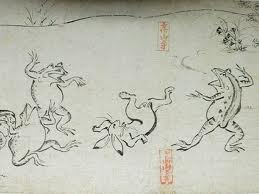
\includegraphics[scale=0.7]{emakimono.jpg}
\end{center}

\paragraph{} Au XIX\ieme siècle, le Japon subit une vague d'occidentalisation
tandis que les journaux satiriques se développent de plus en plus en occident.
C'est à cette époque que le manga s'industrialise. Au XX\ieme siècle, des séries
apparaissent dans les journaux quotidiens et de nouveaux magazines pour enfants
consacrés aux mangas sont créés tels que les périodiques \underline{Shônen
Club} en 1914 et \underline{Shôjo Club} en 1923.

\section{La naissance du manga moderne}

\paragraph{} Au lendemain de la Seconde Guerre Mondiale, les mangas se sont
multipliés pour répondre à une forte demande de distraction bon marché. De
plus, les comics arrivant au Japon inspirent les auteurs japonais.

\paragraph{} L'un des auteurs les plus marquants de cette époque fut Osamu
Tezuka. Il publie son premier manga en 1946. Il rêve de se lancer dans le
dessin animé mais n'en a pas les moyens. Pour pouvoir animer ses histoires, il
crée un style graphique et de mise en page dans le but de faire ressentir les
mêmes émotions que la vision d'un film : il dessine des cases de tailles et de
forme variable pour donner une dynamique cinématographique, il dessine la même
action sous de nombreux angles différents pour donner un impression de ralenti,
il ajoute des traits de vitesse et enfin il fait de grands yeux très expressifs
à ses personnages pour accentuer leurs sentiments et leurs émotions. Cette
technique fut ensuite utilisée par tous les autres auteurs jusqu'à aujourd'hui.

\begin{center}
	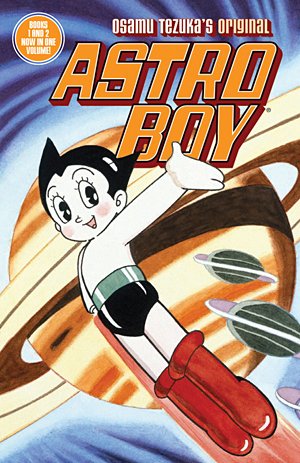
\includegraphics[scale=0.4]{astroboy.jpg}
\end{center}

\paragraph{} En 1962, Tezuka crée le Studio Mushi où il adapte ses succès en
anime. Il installe ainsi le système impliquant qu'un manga à succès est
généralement adapté en anime.

\section{L'introduction du manga en France}

\paragraph{} À la fin des années 70, la production européenne de dessin anime
est insuffisante pour répondre à la demande. Les grandes chaines se tournent
alors vers les productions japonaises qui sont nombreuses, variés et peu chère.

\paragraph{} Ainsi, en 1978, Antenne 2 diffuse \underline{Goldorak} qui eut un
succès inattendu considérable. En effet, la série eut même droit de faire la
couverture de Paris Match intitulée ``la folie Goldorak''.  Suite à ce succès,
Antenne 2 acquière et diffuse trois autres série : \underline{Albator},
\underline{Capitaine Flam} et \underline{Candy}.

\begin{center}
	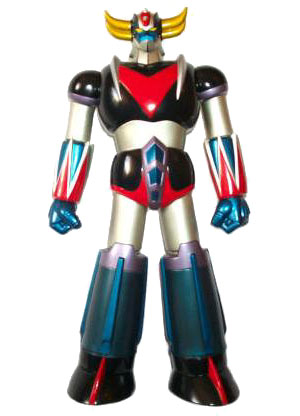
\includegraphics[scale=0.4]{goldorak.jpg}
\end{center}

\paragraph{} En 1983, Antenne 2 diffuse \underline{Les Mystérieuses Cités D'OR}
qui est une réalisation conjointe des studios français, luxembourgeois et
japonais.

\paragraph{} Face au succès des animes japonais sur Antenne 2, La Cinq commence
a diffusé ses propres animes japonais tels \underline{Jeanne et Serge} en 1987
et \underline{Olive et Tom} en 1988. Enfin, TF1 crée l'émission le Club
Dorothée dans laquelle elle diffuse les plus gros succès du moment au Japon :
\underline{Saint Seiya}, \underline{Ken le Survivant} et \underline{Dragon
Ball}.

\section{La polémique \underline{Ken le Survivant}}

\paragraph{} Cependant ces animes venu du Japon font polémique. En effet, en
1989, Ségolène Royal publie \underline{Le Ras-le-bol des bébés zappeurs} dans
lequel elle reproche aux animes japonais de montrer une trop grande violence.
Ses propos illustrent les préjugés forgés à l'époque.

\begin{center}
	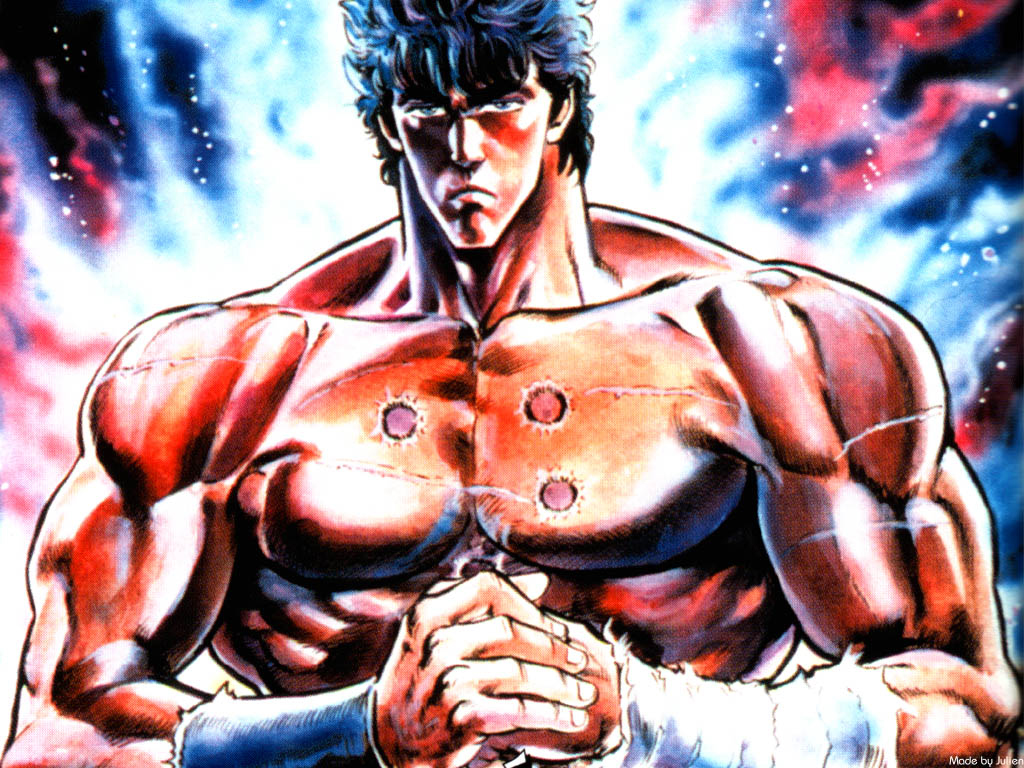
\includegraphics[scale=0.15]{ken.jpg}
\end{center}

\paragraph{} L'anime le plus critiqué est \underline{Ken le Survivant}. En
effet, cet anime diffusé parmi les dessins animés pour enfants raconte
l'histoire de Ken qui erre dans un monde post-apocalyptique en aidant les
innocents à se protéger face aux crapules grâce aux arts martiaux. De plus, les
doubleurs Français ont truffé la version française de jeux de mots plus ou
moins intelligent.

\section{Des années 90 à aujourd'hui}

\paragraph{} En 1993, le Club Dorothée diffuse \underline{Dragon Ball Z} qui
rencontre un  succès tel qu'il sera ensuite diffusé sous format papier. De nos
jours, les animes sur les chaines généralistes ne sont que les rediffusions des
grands succès du début des animes japonais en France.  En effet, pour trouver
des animes plus récent, il faut passer par la TNT, les chaines spécialisées ou
les chaines payantes.

\section{Le début du manga papier}

\paragraph{} Entre 1978 et 1982, un magazine intitulé \underline{Le Cri Qui
Tue} essaye sans succès de publier des mangas. En 1983, la maison d'édition Les
Humanoïdes Associés tentent de publier \underline{Gen d'Hiroshima} mais le
public n'est pas au rendez-vous.

\paragraph{} En 1988, Jacques Glénat rentre du Japon avec un manga intitulé
\underline{Akira} qu'il juge très prometteur. Il apparait d'abord en 1990 sous
forme de fascicule couleurs mais ne rencontre pas le succès. En 1991, la sortie
du film tiré de ce manga va éveiller un vif intérêt des Français envers l'art
des mangakas. Glénat publie ensuite \underline{Akira} dans un format livre de
poche ayant ainsi un grand succès.

\begin{center}
	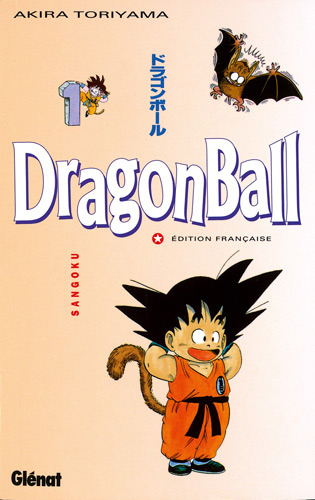
\includegraphics[scale=0.3]{dragonball.jpg}
\end{center}

\paragraph{} Mais les mangas en version papier connaissent un véritable succès
seulement avec la sortie de \underline{Dragon Ball} en 1993. Suite à ce succès,
en 1995, Casterman lance sa collection manga et Dargaud crée sa filiale Kana.
Il existe 	aujourd'hui trente-trois éditeurs spécialisé en France.

\section{Les films d'animation}

\paragraph{} Le plus grand honneur pour un mangaka c'est de voir son manga
adapté en anime puis en film d'animation. Le premier film d'animation tiré d'un
manga qui est sorti en France fut \underline{Akira} en 1991. Puis le film
\underline{Ghost In The Shell} de Mamoru Oshii sort en 1997. Sa suite,
\underline{Innocence}, est sélectionnée au festival de Cannes en 2004.

\paragraph{} En 1995, \underline{Porco Rosso} de Hayao Miyazaki sort au cinéma
en France. Mais c'est en 2000 que Miyazaki conquis le public français avec
\underline{Princesse Mononoké}. Suite au triomphe du \underline{Voyage de
Chihiro}, les anciens films de Miyazaki sont diffusés en France.

\begin{center}
	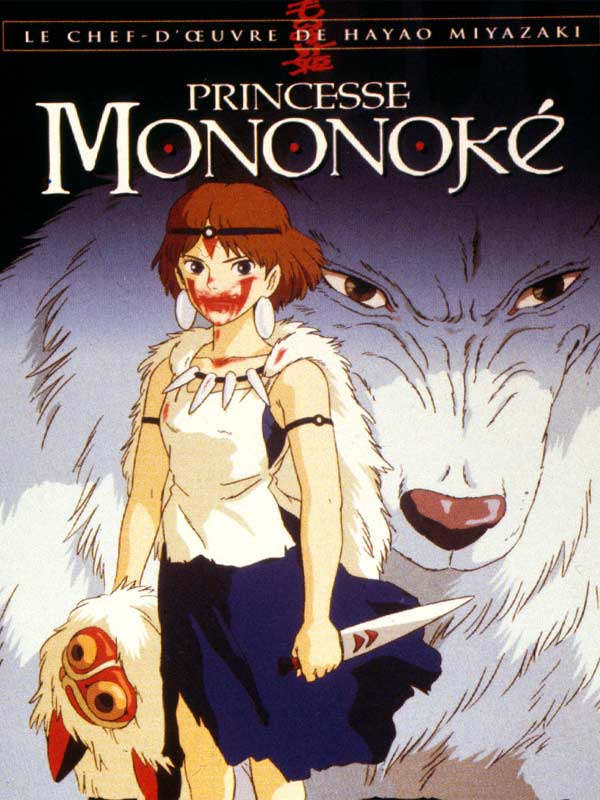
\includegraphics[scale=0.2]{miyazaki.jpg}
\end{center}

\paragraph{} En 2003, sort \underline{Interstella 5555} qui est une mise en
scène de l'album ``Discovery'' de Daft Punk par Leiji Matsumoto le créateur
d'\underline{Albator}.

\section{Les raisons d'un tel succès}

\paragraph{} À l'origine, les œuvres japonaises ont été introduites en France
pour satisfaire un public d'enfants. Cependant, elles ont très vite intéressées
les adolescents.

\paragraph{} Cet engouement peut s'expliquer par un tout nouveau type de
réalisation : la mise en scène est dynamique et cinématographique. En effet, il
y a une alternance continue entre les différents types de cadrages tels que des
gros plan sur les visages, les plans larges pour découvrir le décor, des
mouvements de caméra et la technique du face à face entre deux personnages
présentant sur le même plan le dos d'un personnage et la face d'un deuxième
personnage.

\paragraph{} De plus, les scénarios innovants rendent les mangas très
attrayant. En effet, les séries se suivent comme des feuilletons ce qui permet
de développer des scénarios complexes. Les personnages ont des psychologies
très développées et qui évolue tout au long de la série suite aux expériences
qu'ils traversent. Enfin, il arrive qu'il y ait des flashbacks lorsqu'un
personnage se remémore un évènement ce qui permet aux spectateurs ou lecteurs
de comprendre l'histoire même s'ils ont loupés un épisode.

\paragraph{} Les mangas sont également adaptés au public visé : il existe des
Shônen pour les jeunes garçons qui mettent en scène des affrontements entre les
personnages, des Shôjo pour les jeunes filles qui regroupent des histoires de
romances, de jeunes filles aux pouvoirs magiques et de jeunes sportives. Ce
genre eut un véritable succès grâce à un manque de concurrence au sein des
bandes dessinées belges. En effet, les thèmes abordés sont nouveaux, les
personnages sont souvent des adolescents et le rythme de publication soutenu
permet au personnage de vieillir avec le lecteur ce qui permet au lecteur de
s'identifier au personnage. Il existe d'autres genres tels que les Seinen ou
les Josei destiné aux jeunes adultes et dont les thèmes sont plus matures et la
violence plus crue.

\begin{center}
	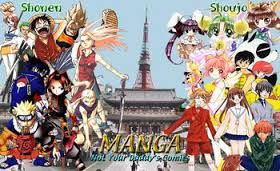
\includegraphics[scale=0.8]{shojo-shonen.jpg}
\end{center}

\paragraph{} L'aspect de chaque personnage est étudié dans les moindres détails
: les yeux sont toujours assez grands pour être très expressifs et les
chevelures sont d'un style séduisant mais différent pour permettre un
attachement à celui-ci. De plus, les tenues sont plus ou moins réfléchies
suivant le contexte de l'histoire : dans un lycée, les personnages porteront un
uniforme tandis que dans une série historique ou fantastique, les tenues seront
réfléchies au détail près.

\paragraph{} Enfin, l'impression en noir et blanc et le format poche donne un
style épuré et un coût faible à l'œuvre.

\section{Des fans impliqués}

\paragraph{} Dans les années 90 apparait des fanzines autrement dit des
magazines créés par des fans pour des fans. En effet, en 1991 a lieu la
première parution d'\underline{AnimeLand}. Il est encore en activité
aujourd'hui. En 2006, les Humanoïdes Associés crée le \underline{Shogun Mag},
un magazine de prépublication comme il en existe au Japon.

\begin{center}
	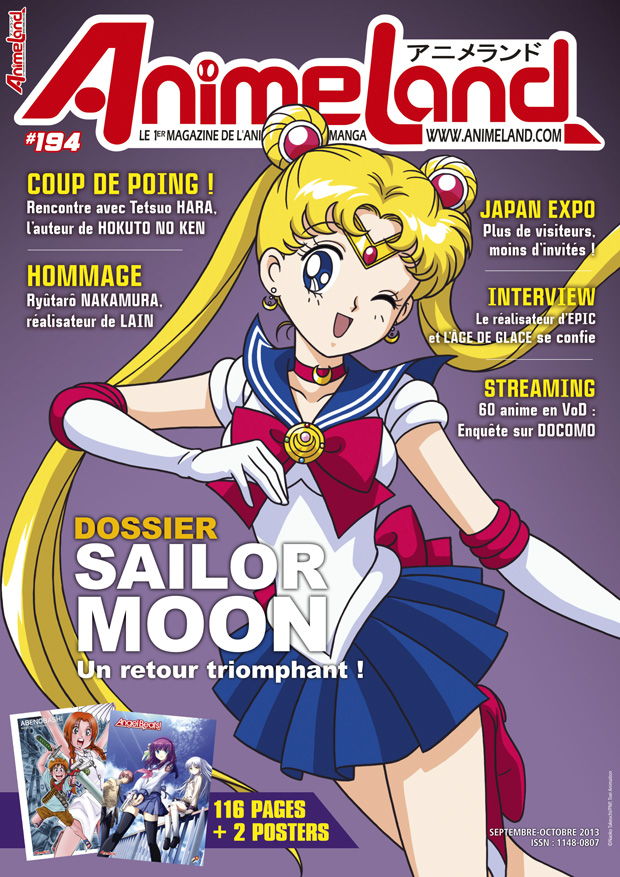
\includegraphics[scale=0.8]{animeland.jpg}
\end{center}

\paragraph{} Internet a aussi permis aux mangas de se propager. En effet, les
fans ont créés les fansubs et les scantrads. Le fansub consiste à se regrouper
en ``team'' pour traduire et sous titrer les animes. Le scantrad, quant-à-lui,
consiste à scanner des mangas papier pour ensuite les traduire. Bien qu'étant
illégal, cette pratique concerne principalement des séries non licenciés en
France ce qui permet de promouvoir et d'évaluer la popularité potentielle de
celles-ci.

\section{Un Japon qui fascine et qui inspire}

\paragraph{} Les mangas permettent aussi de découvrir la culture japonaise. En
effet, les mangas ont tendances à décrire certains aspects de la culture
japonaise.

\paragraph{} En 1999, la Japan Expo est créée. Il s'agit d'un festival
regroupant des stands sur les mangas, les animes, les jeux vidéo, le cinéma, la
J-Music et la culture japonaise. Il permet aussi aux fans de faire du cosplay,
une activité qui consiste à se déguiser comme son personnage favori du moment.

\begin{center}
	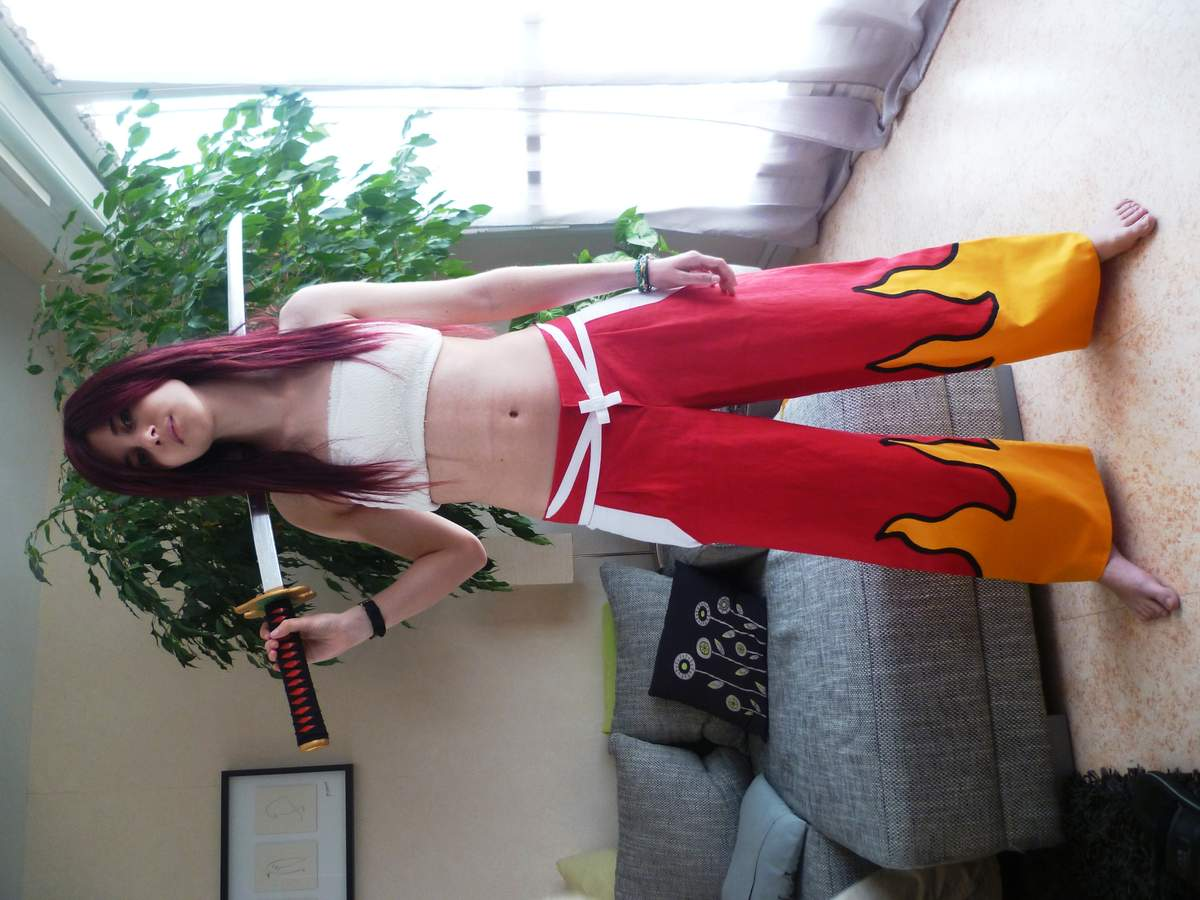
\includegraphics[scale=0.3, angle=-90]{erza.jpg}
\end{center}

\paragraph{} L'art du manga fascine aussi les auteurs de bande dessinée
français. En effet, en 2005, Jean Giraud collabore avec Jirô Taniguchi pour
créer \underline{Icare}. De plus, on assiste à l'apparition de ``manfra'',
mangas français, tels que \underline{Dofus} ou \underline{DreamLand}.

\chapter{Un vocabulaire}

\section{Catégories de manga en fonction du public visé}

\begin{center}
	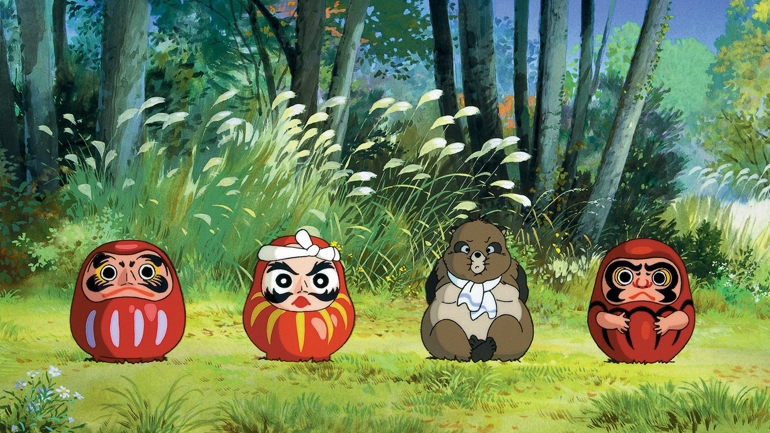
\includegraphics[scale=0.5]{Kodomo.jpg}
\end{center}

\begin{description}
	\item[Kodomo:] Anime ou manga destiné aux jeunes enfants.
	\item[Shonen:] Anime ou manga destiné aux jeunes garçons (spécifiquement
		pour des personnes de moins de 14 ans mais qui peut avoir une audience
		beaucoup plus large).
	\item[Shojo:] Anime ou manga destiné aux jeunes filles.
	\item[Seinen:] Anime ou manga destiné aux hommes qui sont dans les environs
		de la 50aine.
	\item[Josei:] Anime ou manga destiné aux femmes allant de la fin de
		l'adolescence à la femme adulte.
	\item[Ecchi:] Anime, manga ou jeu érotique.
	\item[Hentai:] Anime, manga ou jeu pornographique.
\end{description}

\section{Catégorie de manga en fonction de l'univers}

\begin{center}
	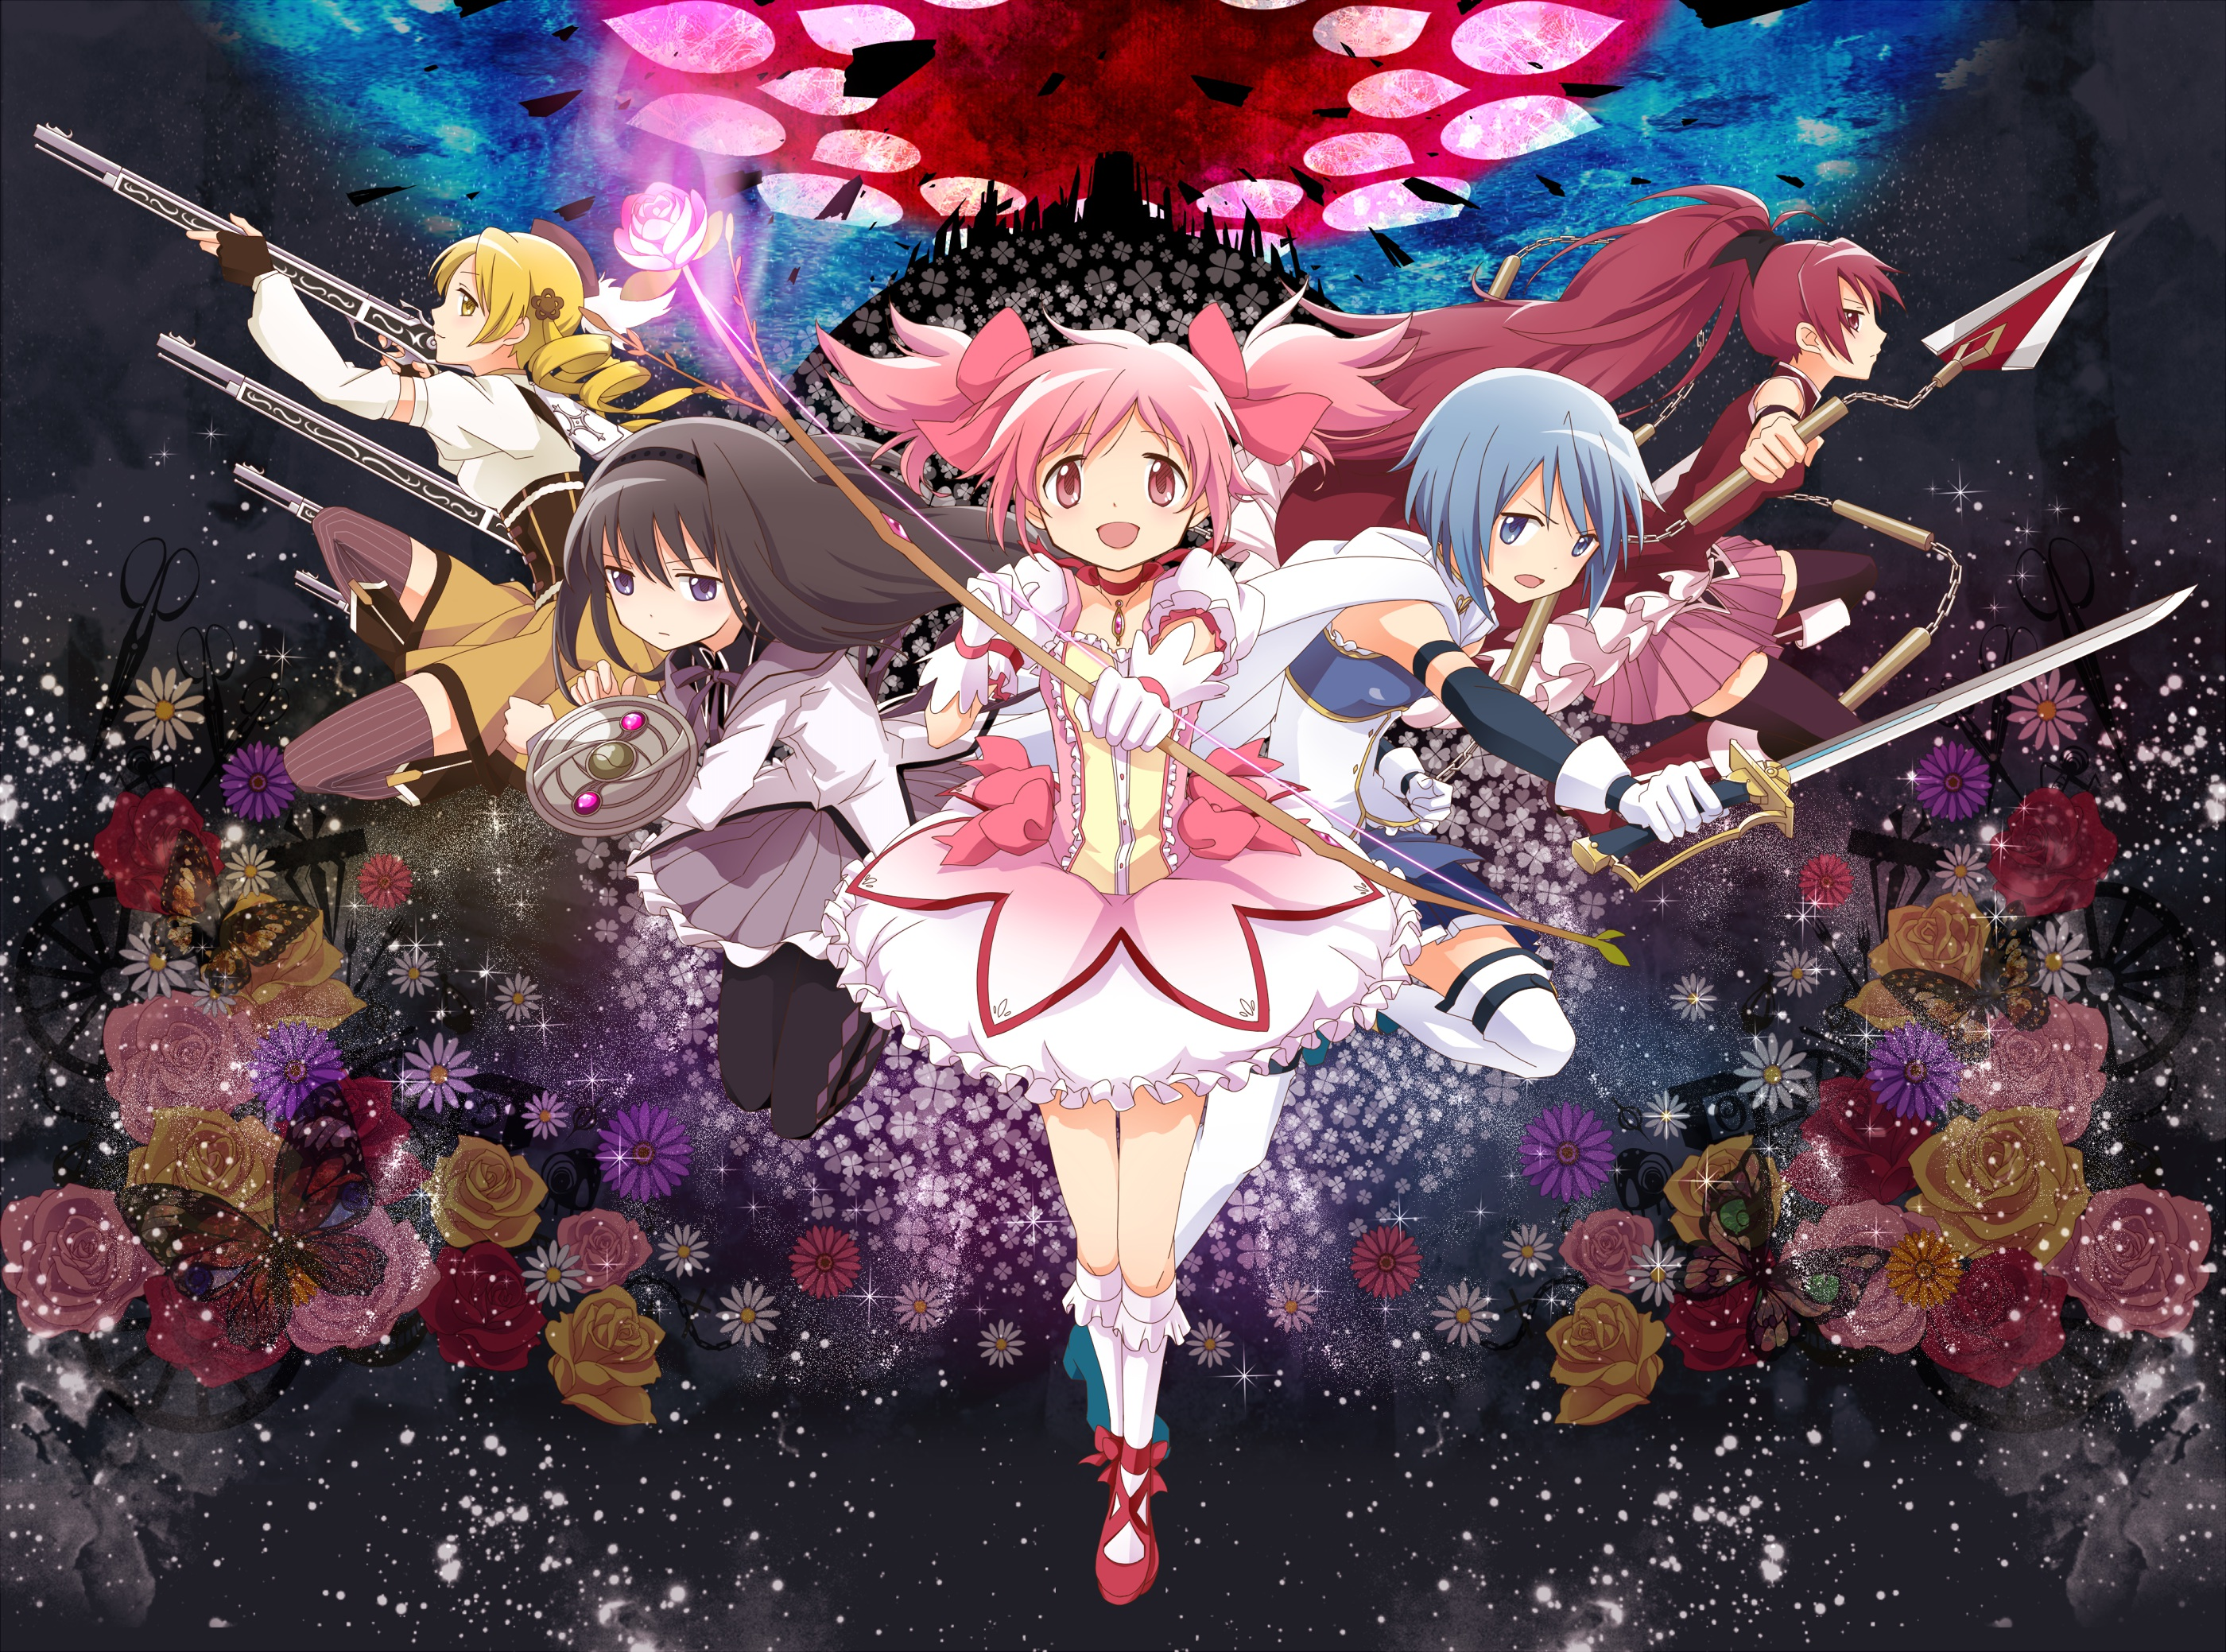
\includegraphics[scale=0.8]{Madoka.jpg}
\end{center}

\begin{description}
	\item[Magical girl (Mah\=o Sh\=ojo):] Manga ou anime mettant en scène de
		jeunes filles ayant des pouvoirs magiques, généralement de type
		sorcière ou magicienne (Par exemple: Madoka$\star$Magika, Sailor Moon).
	\item[Harem:] Manga ou anime ayant un personnage masculin proéminent pour
		un nombre plus important de personnages féminins principaux.
	\item[Mecha:] Manga ou anime mettant en scène des ``mecha'', à savoir des
		robots humanoïdes de taille gigantesque (Par exemple: Neon Genesis
		Evangelion, Goldorak)
\end{description}

\section{Suffixes honorifique}

\begin{description}
	\item[San:] Niveau de politesse standard (équivalent à Mr./Mme.)
	\item[Kun:] Très souvent utilisé pour s'adresser à des garçons ou des amis
		masculins.
	\item[Chan:] Utilisé pour les bébés, jeunes filles ou jeunes garçons, ou
		pour les petits-amis/amis très proches.
	\item[Sensei:] Utilisé pour les professeurs, politiciens, docteurs ou
		autres personnes d'autorité.
	\item[Sama:] Utilisé pour les divinités et les personnes de la royauté.
	\item[Senpai:] Utilisé pour les supérieurs ou les personnes respectées.
\end{description}

\section{Caractère type de personnages}

\begin{center}
	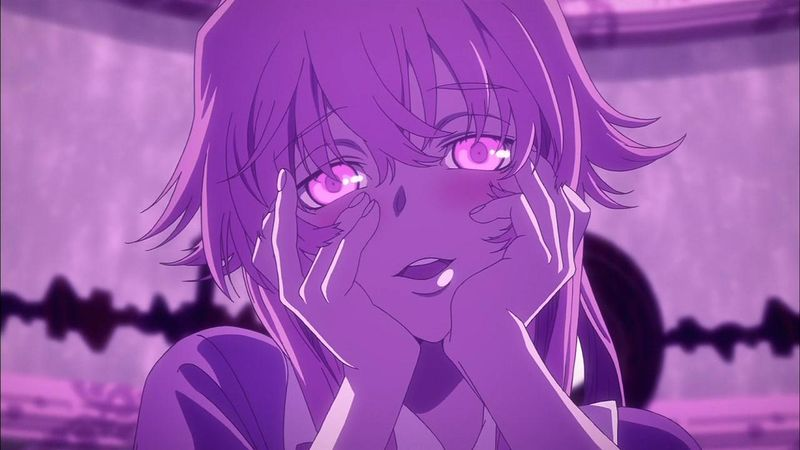
\includegraphics[scale=0.5]{Yandere.jpg}
\end{center}

\begin{description}
	\item[Yandere:] Personnage psychologiquement instable ayant des
		sentiments pour un autre personnage mais utilisant ses pulsions
		meurtrières pour par exemple ``se débarrasser de la compétition''.
	\item[Tsundere:] Personnage dur et énervant au premier abord mais
		affectueux une fois sortie de sa coquille.
	\item[Kuudere:] Personnage froid et cynique en apparence mais attentionné
		en réalité.
	\item[Deredere:] Personnage adorable et énergique envers tout le monde.
	\item[Dandere:] Personnage calme et silencieux lorsque entouré par
		plusieurs personnes mais adorable et énergique lorsque seul avec une
		autre personne.
	\item[Kamidere, Himedere, Oujidere:] Personnage ayant un complexe
		de supériorité et se croient respectivement l'équivalent d'un
		Dieu (Kami), Princesse (Hime) ou Prince (\=Oji).
\end{description}

\section{Style de dessins}

\begin{center}
	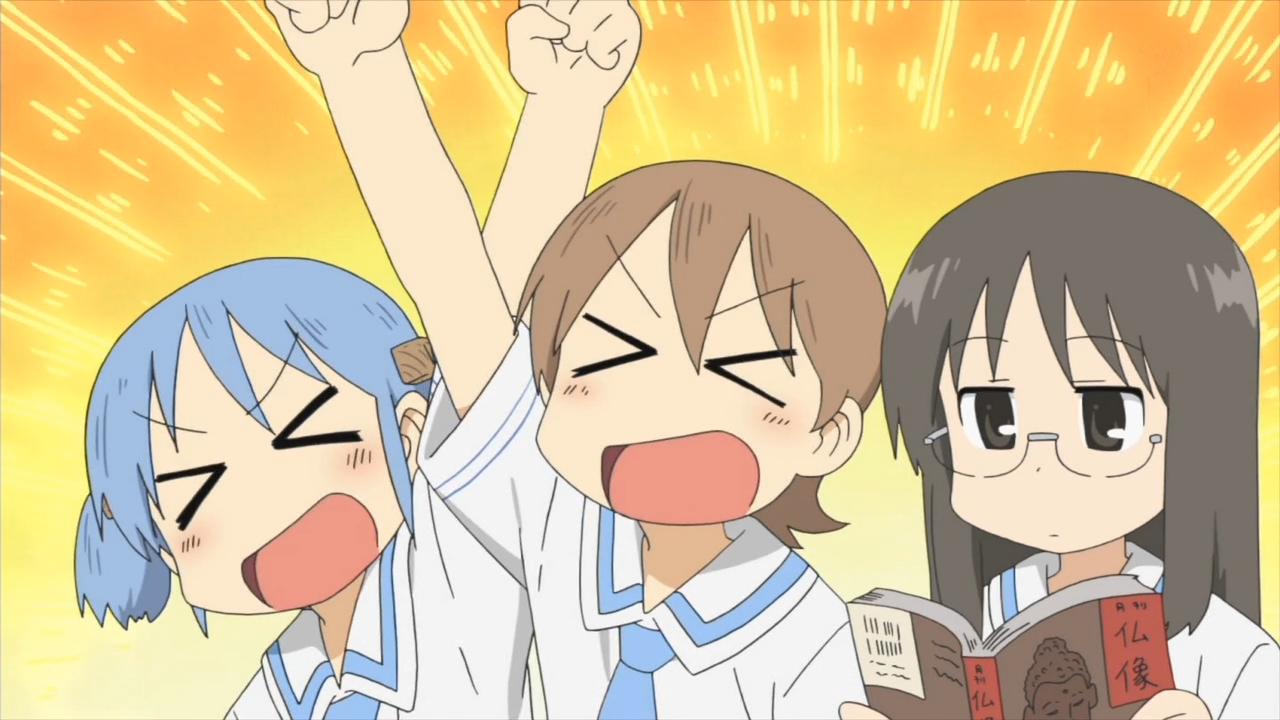
\includegraphics[scale=0.3]{Moe.png}
\end{center}

\begin{description}
	\item[Moe:] Style de dessin caractéristique et simpliste qui a pour but de
		faire sentir des sentiments d'affection envers les personnages (Par
		exemple: Nichijou).
\end{description}

\section{Idéalisation}

\begin{center}
	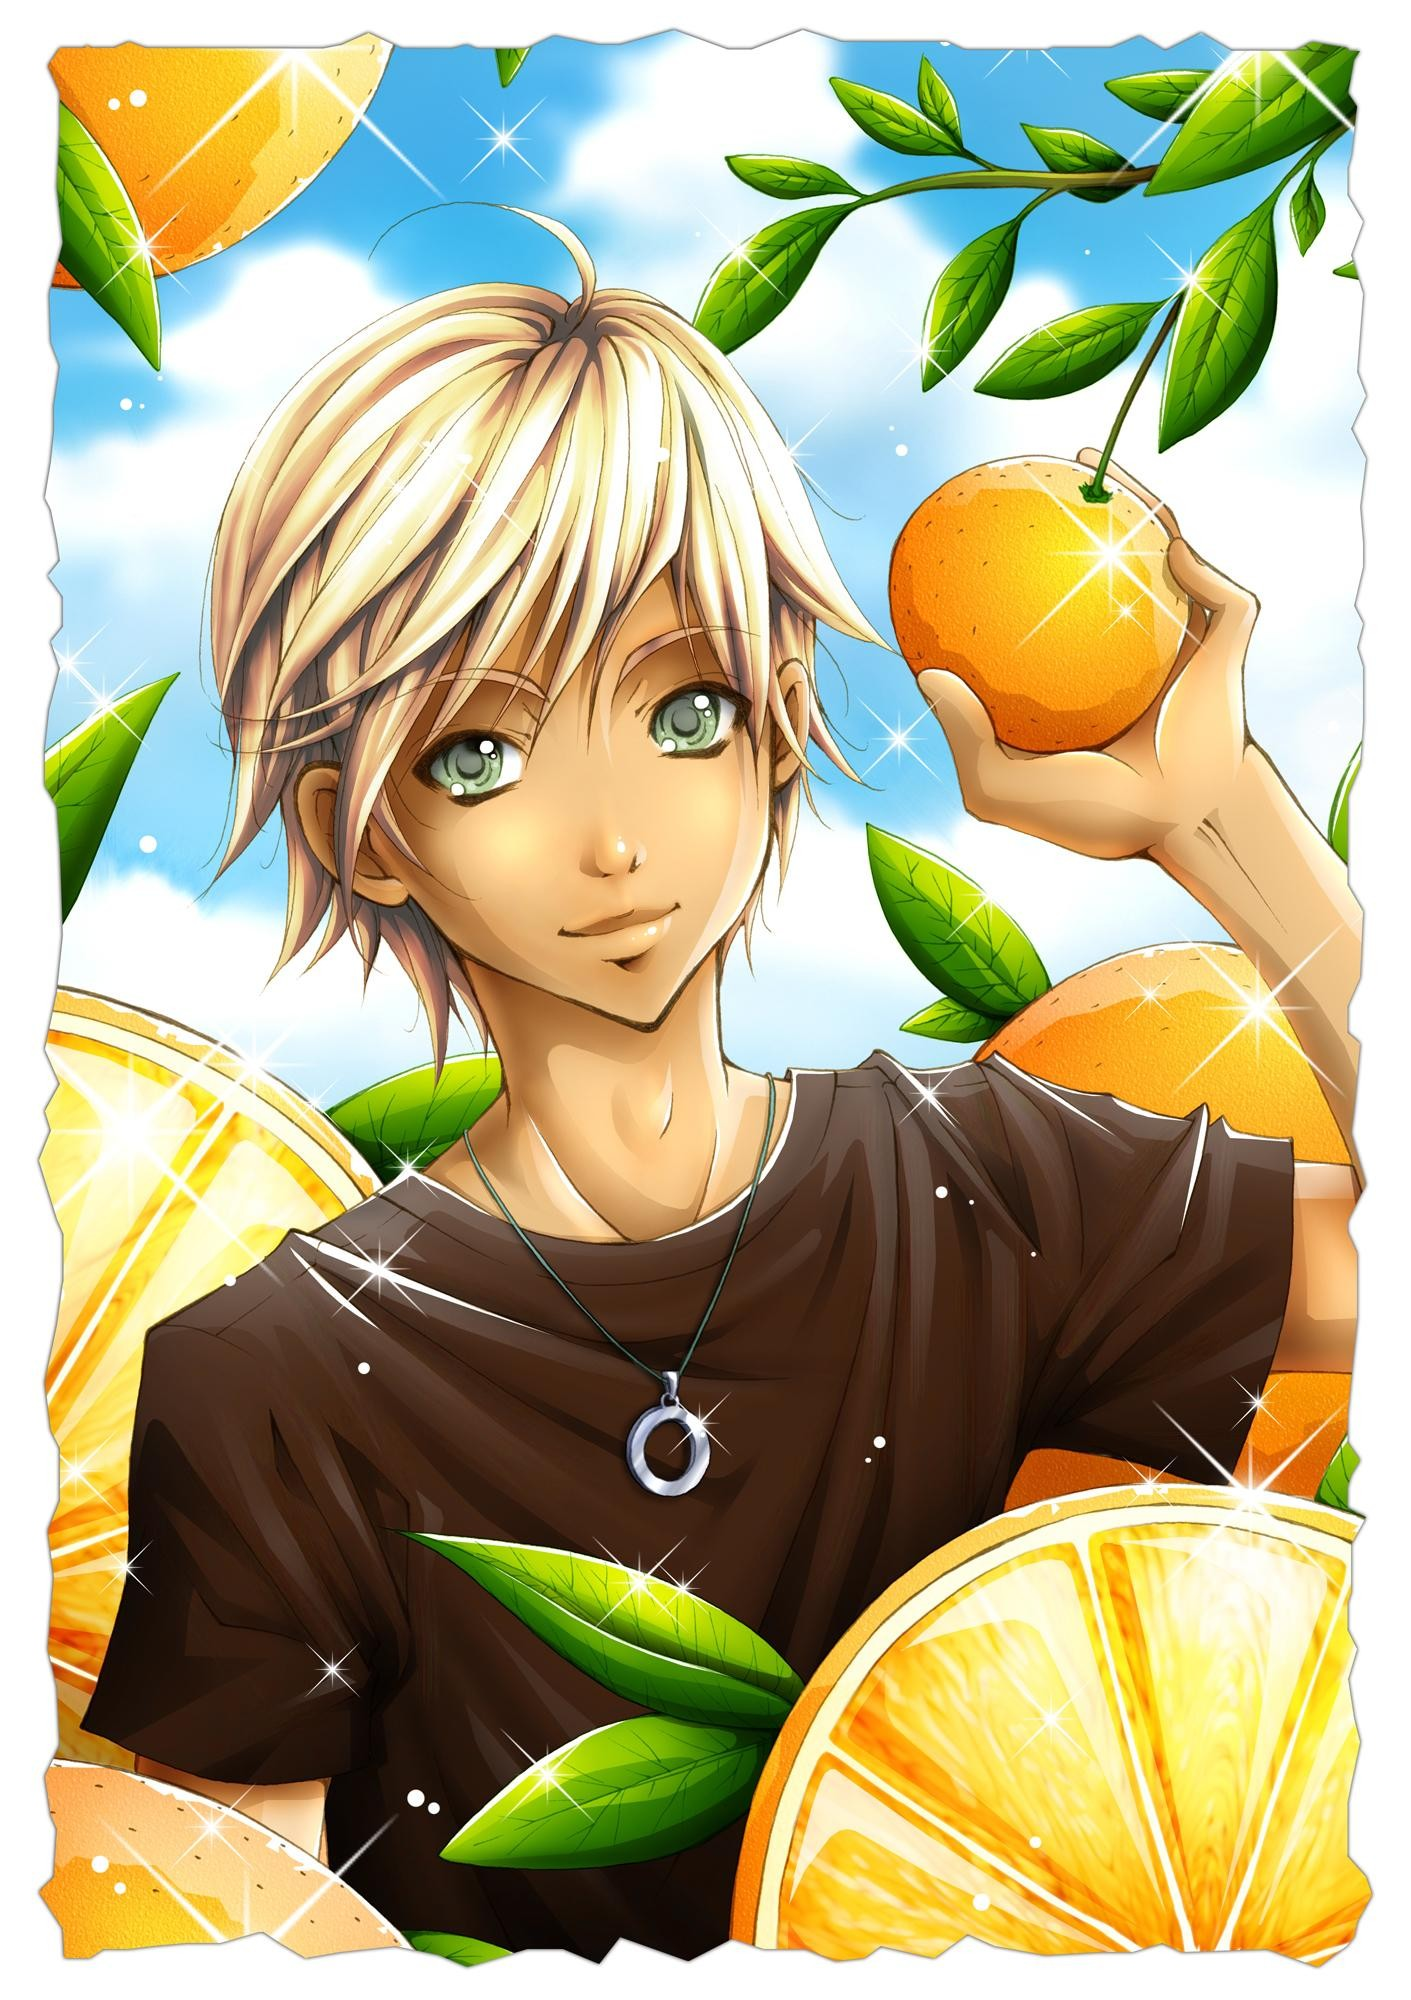
\includegraphics[scale=0.15]{Bishounen.jpeg}
\end{center}

\begin{description}
	\item[Bishonen:] Représentation de l'idéal masculin, en majorité un garçon
		efféminé, androgyne et jeune.
	\item[Bishojo:] Représentation de l'idéal féminin.
\end{description}

\chapter{Les produits dérivés}

\section{Le marché des produits dérivés}

\paragraph{} Les produits dérivés des Otakus sont très nombreux et ne cessent
de se démultiplier. Depuis le 21ème siècle, on considère qu'être Otaku relève
d' une passion qui se démocratise énormément dans le monde, mais en priorité au
japon. La société japonaise l'a bien compris et le marché aussi. En effet, le
marché des objets dérivés au Japon est ainsi égal à celui des contrats de
diffusion des œuvres dont ils sont tirés, représentant plus de 1.000 milliards
de yens (7,5 milliards d'euros) par an.

\paragraph{} En effet, ils se sont adapté en renforçant davantage l'offre
chaque année, car le phénomène se répand et d'énorme flux d'argent est véhiculé
par ce mouvement très prometteur.

\paragraph{} Différente forme de produit dérivé existe. Des t-shirts aux
figurines. Des posters aux stickers. Des mugs aux portes-clés. Mais aussi des
articles de papeterie, des bijoux ou des DVD.

\begin{center}
	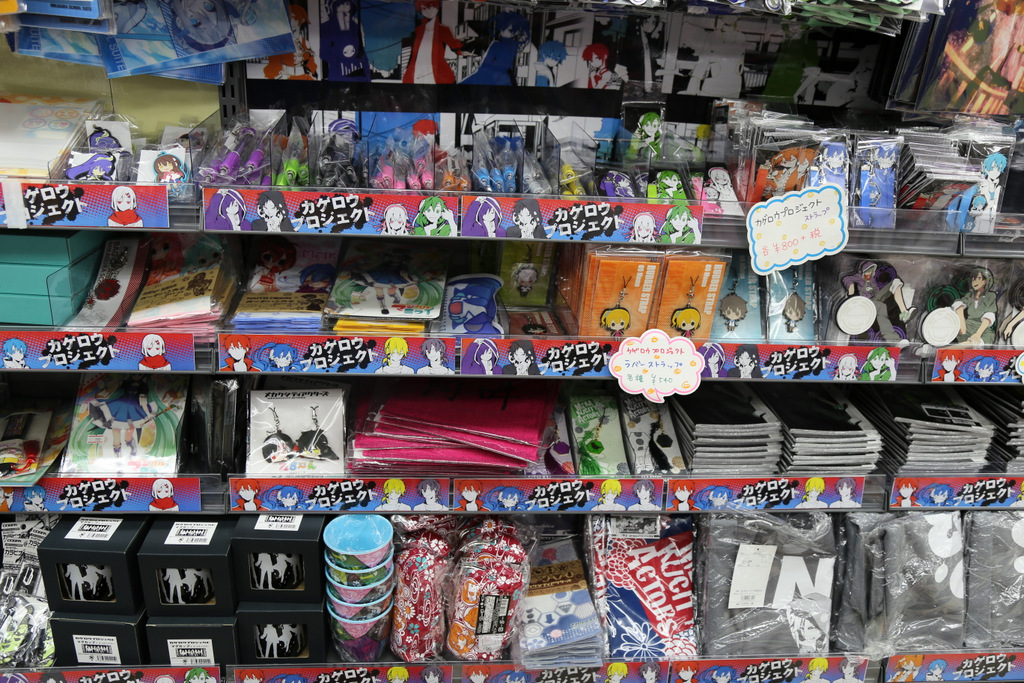
\includegraphics[scale=0.15]{produit.jpg}
\end{center}

\section{La différence entre le Japon et la France}

\paragraph{} Au japon, nous pouvons distinguer l'ampleur du mouvement bien plus
grand que dans les autres pays, qui est en relation avec la vie professionnelle
japonaise. La culture japonaise se veut très stricte concernant le travail, par
exemple la signature d'un contrat de travail représente pour un japonais un
événement majeur de sa vie, car le travail correspond à un engagement tel le
mariage et donc à une promesse de fidélité semblable au serment d'alliance.
L'employé doit porter le costume de l'entreprise et être conditionné par les
valeurs que l'entreprise veut véhiculer.

\paragraph{} Ainsi, pour ces raisons, les Japonais considèrent le gadget et le
produit dérivé comme une manière se distinguer, de s'exprimer, de sortir de
l'anonymat des villes surpeuplées.

\paragraph{} On peut noter une petite exception pour Pokemon qui a connu un
succès incroyable à l'étranger et en France.

\begin{center}
	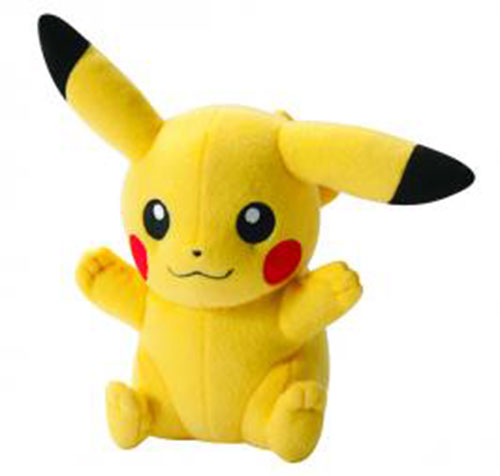
\includegraphics[scale=0.15]{pokemon.jpg}
\end{center}

\chapter{Les conventions}

\section{L'origine des conventions}

\paragraph{} Les rencontres dédiées aux mangas et anime sont anciennes au
Japon. Une pionnière du genre est Comiket, créée en 1975 à Tokyo dans le but de
populariser des d\=ojinshi, mangas créés et publiés par des fans. Elles se
multiplient au fil des années avec l'aide des éditeurs, qui y voient un bon
moyen d'assurer la publicité de leurs séries.

\paragraph{} Le phénomène se développe également en Occident dans les années
1980 avec l'importation de la culture japonaise. Aux États-Unis, ces anime
conventions rejoignent les festivals de culture populaire américaine :
science-fiction, comic books, etc.. Leur véritable succès ne commencera
toutefois que dans les années 1990, décennie durant laquelle de tels évènements
apparaissent aussi en Europe. En France, la plus célèbre est Japan Expo, créée
en 1999, qui lance pour de bon le phénomène des conventions françaises
(l'anglicisme convention ayant été adopté pour les différencier des expositions
plus classiques). D'autres évènements suivent la tendance : Paris Manga, Japan
Expo Sud\ldots Leur point commun est que leur croissance rapide les a poussés à
s'ouvrir à une culture geek plus générale, invitant des créateurs de séries,
jeux vidéo, films de SF, etc.

\begin{center}
	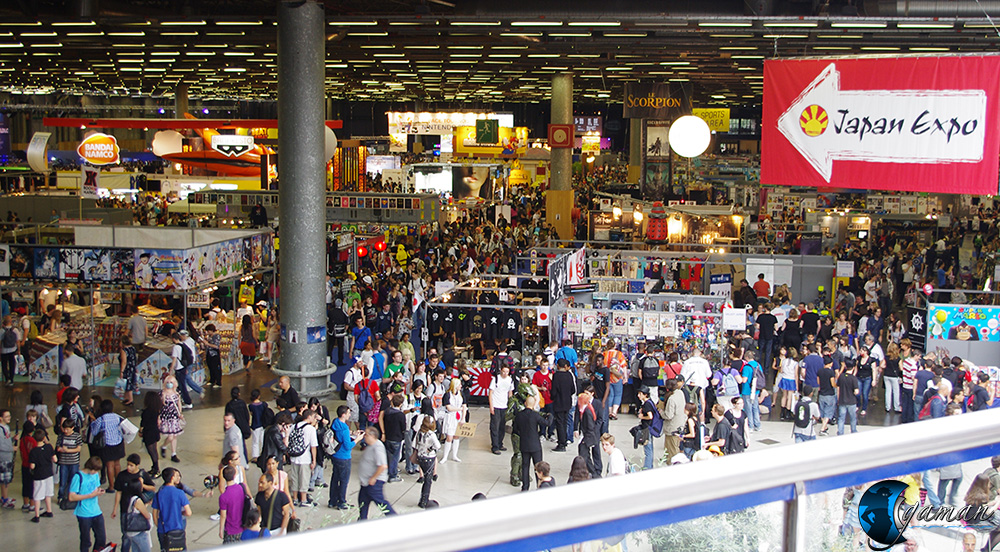
\includegraphics[scale=0.3]{japanexpo.jpg}
\end{center}

\section{Le contenu des conventions}

\paragraph{} Les invités d'honneur sont au centre de ces évènements : il peut
s'agir d'un mangaka, d'un scénariste ou d'un designer célèbre présent pour des
dédicaces ou une conférence. Ils peuvent également tenir un atelier. De
nombreux autres artistes tiennent des stands de dédicace. Ceux-ci sont parfois
tenus par un éditeur occidental, qui compte sur la présence des artistes pour
faire découvrir une série en vue d'une publication.

\paragraph{} On y trouve aussi de nombreux stands de vente, où sont proposés
des mangas mais également de nombreux produits dérivés : peluches, posters, et
même épées. Il est rare de revenir d'une convention sans un ou deux goodies.

\begin{center}
	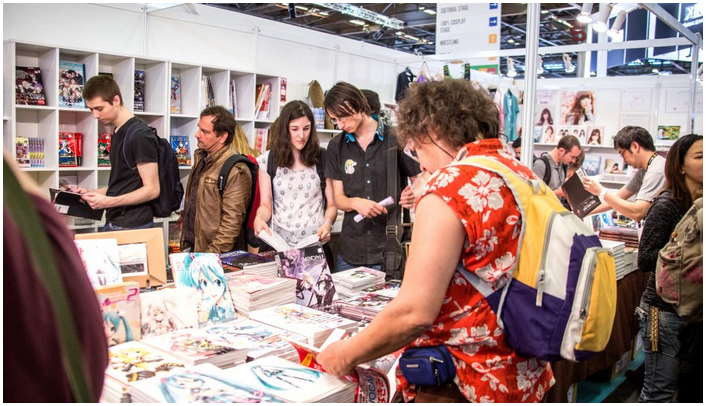
\includegraphics[scale=0.5]{boutique.png}
\end{center}

\paragraph{} Les salles de conférence sont également employées pour des
avant-premières et projections tests, souvent suivies de panels où des artistes
répondent aux questions des fans. Des concours y ont également lieu, notamment
de cosplay, discipline chère aux conventions. Les fans y trouvent un moyen
d'exprimer leur créativité en confectionnant des tenues inspirées ou
directement reprises de celles de personnages de mangas ou jeux vidéo. Le
phénomène est sans doute celui dont la croissance a été la plus sensible ces
dernières années, parfois au regard moqueur des médias généralistes.

\begin{center}
	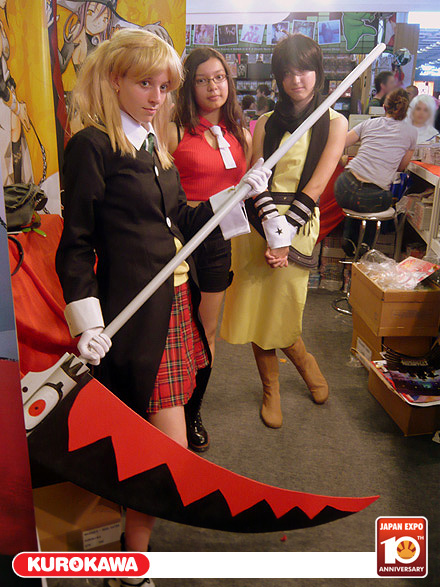
\includegraphics[scale=0.3]{cosplay.jpg}
\end{center}

\paragraph{} Enfin, les conventions proposent des expositions : d'art japonais,
de dessins préparatoires, etc.

\begin{center}
	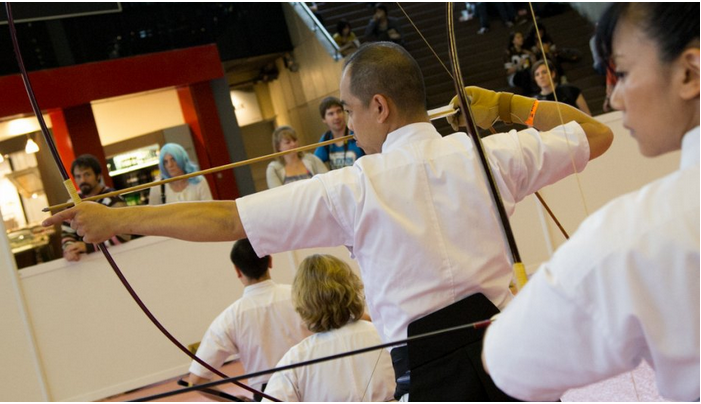
\includegraphics[scale=0.4]{demo.png}
\end{center}

\chapter{Interview de deux Otakus}

\paragraph{} Nous avons interviewé deux personnes passionnés de mangas ou animes
dont nous ne divulgueront pas les noms. Nous les appellerons donc A et B.\\
\\

\textbf{Depuis quand lis-tu des mangas/regardes tu des animes?}\\
A: Je regarde des animes depuis environ 1 ans et demi. Je n'ai jamais lu de
mangas.\\
B: Je lis des mangas depuis l'âge de 9 ans mais j'ai commencé à regarder des
animes à l'âge de 6 ans.\\

\textbf{Quel fut ton premier manga/anime?}\\
A: Le premier anime que j'ai regardé été \underline{Naruto}.\\
B: Le premier anime que j'ai vu été \underline{Olive et Tom} à la télé et le
premier manga que j'ai lu été \underline{Dragon Ball}.\\
\\
\textbf{Quel type d'animes/mangas lis-tu en général?}\\
A: Je regarde tous les genres: shojo, shonen, seinen...\\
B:Je regarde et lis beaucoup de genres différents: de la science fiction, du
sport, de la fantasy\ldots\\
\\
\textbf{Qu'est-ce qui t'attire dans les mangas/animes?}\\
A: C'est la folie du genre qui m'as attiré dans les animes.\\
B: Ce qui m'a attiré dans les mangas et les animes c'est leur capacité de
rendre génial un sujet stupide.\\
\\
\textbf{Quel est ton manga/anime favori?}\\
A: Je dirai que mon anime préféré est \underline{FullMetal Alchemist
Brotherhood}.\\
B: Je ne pourrai pas citer un anime/manga en particulier: il y en a trop de
bien.\\
\\
\textbf{Préfères-tu les mangas ou les animes? Pourquoi?}\\
A: Je ne lis jamais de mangas, je ne regarde que des animes.\\
B: Je préfère les mangas, je trouve que les animes commencent à manquer
d'originalité: ils se ressemblent de plus en plus.\\
\\
\textbf{Préfères-tu la VO ou la VF pour les animes?}\\
A: Ben la VO.\\
B: La VO.\\
\\
\textbf{As-tu vu des films d'animation japonais? Combien? De quel réalisateur?}\\
A: Au moins une dizaine du studio Ghibli.\\
B: Oula plein.\\
\\
\textbf{Es-tu déjà allé à une convention? Laquelle? Combien de fois? Qu'est-ce qui t'as plu?}\\
A: Non jamais.\\
B: J'y vais à chaque fois que je peux. J'ai souvent fait la Japan Expo et
parfois Paris Manga. Mais comme ça coute cher je n'ai fait que des conventions
sur Paris.\\
\\
\textbf{As-tu déjà fait du cosplay?}\\
A: Oui, une fois en Pikachu.\\
B: Jamais.\\
\\
\textbf{Lis-tu des scans ? Regardes-tu en streaming ou téléchargement?}\\
A: Je ne regarde qu'en streaming ou téléchargement.\\
B: Je commence souvent mes séries en scan pour les découvrir mais parfois je
les achète car je trouve que certaine série mérite qu'on possède tous les tomes
chez soi.
